\section{Model evaluation} \label{sec:model_evaluation}

% The Unet, small Unet, ResUnet and c-ResUnet architectures were evaluated and compared based on both detection and counting performance. 
All the presented approaches were evaluated and compared based on both detection and counting performance. 
Also, ablation studies were conducted to assess the impact of artifacts oversampling and weight maps.
% Also, ablation studies assessed the impact of artifacts oversampling and weight maps.

In order to evaluate the detection ability of the models, a dedicated algorithm was developed.
% Specifically, each target cell was compared to all objects in the corresponding predicted mask and uniquely associated with the closest one.
Specifically, each predicted object is compared to all cells in the corresponding ground-truth label and uniquely associated with the closest one.
If the distance between their centroids is less than a fixed threshold (50 pixels, i.e. average cell diameter), the predicted element is considered a match and it increases the true positive count (TP).
% ; a false negative otherwise (FN).
At the end of this procedure, all true objects without matches are considered false negatives (FN). Likewise, the remaining detected items not associated with any target are considered false positives (FP).
Algorithm \ref{algo:pseudocode_metrics} reports the pseudocode of the procedure described above\footnote{full implementation \githubmetrics}.
\begin{algorithm}%[H]
% \begin{algorithmic}[1]
    \DontPrintSemicolon
    % init
    \KwIn{ pred$_i$, mask$_i$}
    \KwOut {TP, FP, FN}       
    % \tcp*{true positives, false positives, false negatives}
    
    Set TP, FP, FN = 0
    
    Get predicted objects, pred\_objs$^i$
    \tcp*{detected cells}
    
    Get true objects, true\_objs$^i$
    \tcp*{annotated cells}
    
    % centers
    Get predicted centers, pred\_ctrs$^i$
    %  \tcp*{centers of predicted objects}
    
    Get true centers, true\_ctrs$^i$
    %  \tcp*{centers of true objects}
    
    \For{each ctr$_j$ in pred\_ctrs$^i$} 
        {
        \tcc{loop over predicted centers}
        \For{each ctr$_k$ in true\_ctrs$^i$}
            {
            \tcc{loop over true centers}
            
             Compute euclidean distance between ctr$_j$ and ctr$_k$ \label{step:ctrs_distance}
             
             Store distance and indexes
             \label{step:store_distance}
            } 
        
         Compute the minimum, min\_dist$_i$ of the distances stored in step \ref{step:store_distance}
         
        \If{understand}{
            Increase true positives, TP
            
            Remove ctr$_j$ from pred\_ctrs$^i$
            
            Remove ctr$_k$ from true\_ctrs$^i$
        }
        
        }
        
    Compute false negatives as true\_objs$^i$ - TP
    
    Compute false positives as pred\_objs$^i$ - TP
    
\caption{metrics computation for i\emph{-th} image.}
\label{algo:pseudocode_metrics}
\end{algorithm}
Starting from these values, we resort to accuracy, precision, recall and $F_1$ score as indicators of detection performance.
% In terms of detection performance, the $F_1$ score was adopted as the primary indicator. Accuracy, precision and recall were also inspected to have a better understanding of the model ability. 
The definitions of such metrics are reported below:

\begin{align}
% \hskip 2cm
\text{accuracy} &=  \frac{\text{TP}}{\text{TP} + \text{FP} + \text{FN}}
= \frac{\text{1}}{\text{1} + \frac{1}{\text{TP}} \left(\text{FP} + \text{FN}\right)}
\label{eq:accuracy}; \\ 
\text{precision} &=    \frac{\text{TP}}{\text{TP} + \text{FP}}; \\
\text{recall} &=    \frac{\text{TP}}{\text{TP} + \text{FN}}; \\ 
F_1 \text{score} &=  \frac{2 \cdot \text{precision} \cdot \text{recall}}{\text{precision} + \text{recall}}
= \frac{2 \cdot \text{TP}}{2 \cdot \text{TP} + \text{FP} + \text{FN}} 
= \frac{\text{1}}{\text{1} + \frac{1}{\text{2TP}} \left(\text{FP} + \text{FN}\right)}
\label{eq:F1}.
\end{align}
% where TP, FP and FN indicates true positive (cells correctly detected), false positives (cells erroneously detected) and false negatives (cells erroneously missed), respectively. 
Notice that we do not have true negatives in \cref{eq:accuracy} since the prediction of the class ``not cell" is done at the pixel level and not at the object level, so there are no ``non-cell" objects predicted by the model.
The above metrics have the limitation of being dependent on the threshold used for the binarization of the predicted heatmaps. Thus, we also look at the \textit{precision/recall curves} and the corresponding Area Under the Curve (AUC) \cite{hanley1982meaning, mason2002areas} for a more general measure of performance. For this purpose, we consider only test images and repeatedly compute precision and recall for each model, varying the binarization threshold from 0.05 to 1 with steps of 0.05 -- these cutoffs represent quantiles of the grayscale intensity distribution in the case of the non-ML baseline.


Regarding the counting task, the Mean Absolute Error (MAE), Median Absolute Error (MedAE) and Mean Percentage Error (MPE) are used instead. More precisely, let $n_{\text{pred}}$ be the number of detected cells in $i$-th image  and $n_{\text{true}}$ be the actual one. Then, the absolute error (AE) and the percentage error (PE) are defined as:

\begin{align}
% \hskip 2cm
\text{AE} &= \lvert n_{\text{true}} - n_{\text{pred}}\rvert ;\\
\text{PE} &= \frac{ n_{\text{true}} - n_{\text{pred}}}{n_{\text{true}} 
% + \epsilon
}.
\end{align}
% where $\epsilon=10^{-6}$ was added to prevent a vanishing denominator when $n_{\text{true}} = 0$. 
Hence, the above counting metrics are just the mean and the median of the AE and the PE.
Although these quantities are intuitive and straightforward to interpret, they may hide poor performances when the counts' distribution has low variability.
For this reason, we also report the $R^2$ coefficient of determination that represents the percentage of variability explained by the model:
\begin{align*}
% \hskip 2cm
R^2 &= 1 - \dfrac{\text{SS}_{\text{residual}}}
{\text{SS}_\text{total}} \\
 &= \numberthis 1 - \dfrac{ \sum_i^{n} \left( y_i - \hat{y}_i \right)^2}{ \sum_i^{n} \left( y_i - \bar{y} \right)^2 },
\end{align*}
where $y_i$ is the count of the $i$-th image, $\hat{y}_i$ is the corresponding predicted count and $\bar{y}$ is the average count.
Hence, values close to 1 indicate that most of the intrinsic variability of the counts is correctly modeled, whereas lower values (close to 0) are a signal of poor predicting ability.

\subsection{Threshold optimization}

The choice of the optimal cutoff for binarization is based on the $F_1$ score computed on full-size images. In practice, the DL models are evaluated on a grid of values and the best one is selected according to the \textit{Kneedle} method \cite{kneedle}. 
The same is done for the non-ML approach, with the only difference of considering the cutoff yielding the maximum $F_1$ value. 
The resultant thresholds is then used to assess performances on the test set.
Although the ultimate goal is retrieving the counts, we rely on detection performance to enforce accurate recognition and avoid spurious balancing between false positives and false negatives -- which are indistinguishable from the counts.
Also, full-size images (as opposed to crops) are used to simulate better the model performance in a real-world scenario.
\begin{figure}
\centerline{
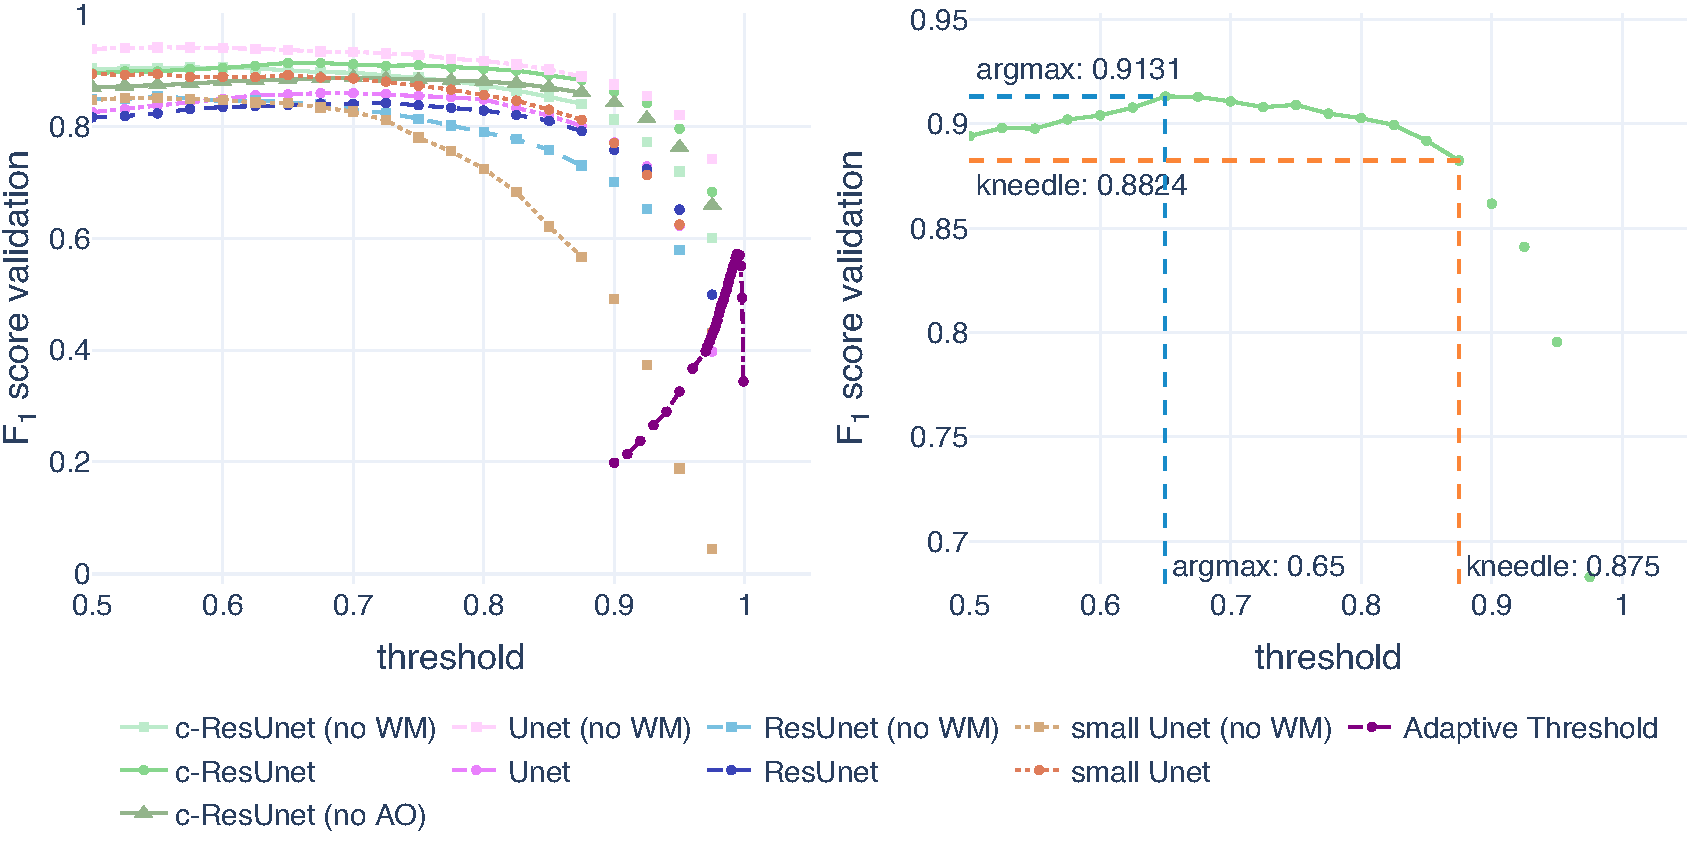
\includegraphics[width=\textwidth]{figures/130_methods/F1_optimization.pdf}
}
\caption{\textbf{Threshold optimization}. On the left, the $F_{1}$ score computed on validation images as a function of the cutoff for thresholding.
On the right, the test $F_1$ score of the c-ResUnet model is used to illustrate the selection of the best threshold for binarization according to \textit{argmax} (blue) and \textit{kneedle} (red) methods.
} 
\label{fig:thresh_opt}
\end{figure}
% If the distance between their centroids was less than a fixed threshold (50 pixels, i.e. average cell diameter), the predicted element was considered a true positive; a false negative otherwise.
% Detected items not associated with any target were considered as false positives instead.

\Cref{fig:thresh_opt} shows the optimization results. On the left, we can see how each model performance varies in the validation set as a function of the cutoff for binarization.
For the adaptive thresholding approach, only very high thresholds lead to acceptable performances and we observe a sharp peak followed by a rapid decrease thereafter.
% Even though lower thresholds work best for all DL models, the $F_1$ curves are rather flat after their peaks. 
On the contrary, all DL models work best for lower thresholds and present $F_1$ curves which are rather flat after their peaks.
Thus, increasing the cutoff allows focusing only on predictions whereby the model is very confident, with just a slight loss in overall performance.
Also, good practices in natural science applications suggest being conservative with counts and only consider clearly stained cells.
For these reasons, we opted for the \textit{argmax} value (0.994) for the baseline approach, while we resorted to the \textit{Kneedle} method \cite{kneedle} for the selection of the optimal DL threshold. 
An example of that choice in the case of c-ResUnet is reported in \cref{fig:thresh_opt} (right).